%!TEX root = ../thesis.tex


\section{Vertical one-sided dual}
\label{s:red}

We can also adapt Fusy's algorithm to generate a vertically one-sided dual. We then need top generate a regular edge labeling without red faces that have $3$ or more edges on both borders.

We will have an additional requirement on top of the requirement that $\ext G$ has no separating triangles. We will also require that $\ext G$ has no separating four cycles.


\mypar{Notational concerns}
  Just as in Section \ref{s:algo} we will use $\C$ to indicate the current sweep line cycle.
  We will repeatedly only consider the path $\cpath$. In that case we will always order it from $\pW$ to $\pE$.

  Instead of interior paths we will consider interior walks but we will use similar notation. That is a walk between two distinct vertices of $\C$ of which all vertices except the first and last one are in the interior of $\C$.

  We will let $\W$ denote a interior walk. Given such a walk of $k$ vertices we index it's nodes $w_1, \ldots, w_k$  in such a way that $w_1$ is closer to $W$ then $w_k$ is (and thus that $w_k$ is closer to $E$ then $w_1$ is).

  Then $w_1$ and $w_k$ indicate the two unique vertices of the walk that are also part of the cycle. We will then let $\restC{\W}$ denote the part of $\C\setminus {\mathrm{S}}$ that is between $w_1$ and $w_k$ (including). $\C_\W$ will denote the closed walk formed when we paste $\restC{W}$ and $\W$.

  Since paths are a subclass of walks all of the above notation can also be used for a path $\P$. Note that the closed walk $\C_\P$ in this case will actually be a cycle.


  We note that the interior of some cycle $\interior(C)$ are all vertices strictly in the interior of this cycle. We will sometimes also take $\interior(C)$ to refer to the induced subgraph of these vertices.

  We let $\intplus(C)$ denote the the vertices of $C$ and $C$'s interior vertices. We will also sometimes let it refer to the subgraph of $G$ induced by these vertices.

  \mypar{Non-crossing walks}
  We will call a walk \emph{noncrossing} if at every vertex $w$ in the walk that is visited $k >1$ times such that $w_{i_1} = w_{i_2} = \ldots = w_{i_k}$ in the walk the clockwise intervals $[w_{i_j-1}, w_{i_j+1}]$ for $j \in \braces {1, \ldots, k}$ are disjoint in the rotation at $w$.
  \fxnote{We might add a (small) figure for clarity (i.e. of a crossing and a non-crossing walk)}

  The nice thing about non-crossing walks is that if they are closed they allow a notion of interior and exterior. We can see this by applying Jordans curve theorem to a version of this walk that is very slightly perturbed at every vertex visited multiple times. Which we can do due to the disjoint intervals in the rotation.

  Hence we can talk about the interior vertices of a closed non-crosing walk.

  \fxwarning{TODO}

  \fxnote{More general for non-crossing paths}


\subsection{The neighbor walk of a path}
  \fxwarning{Note that the same/similar things hold for the left boundary walk}
  During this proof we will frequently use the concept of the left or right neighbor walk of a path.
  Given a path $P = p_1 \ldots p_k$ in a graph $G$
  The \emph{right neighbor walk} $W$ of $P$ will consist of $p_1$ and the vertices adjacent to $p_{2}$ between $p_1$ and $p_{3}$ in the clockwise rotation at $p_{2}$ followed by the vertices between $p_{2}$ and $p_{4}$ in the rotation at $p_{3}$ and so further until we add the vertices between $p_{k-2}$ and $p_k$ in the rotation around $p_{k-1}$ and finally we finish by adding $p_k$ to $W$.
  We then remove all subsequent duplicates from $W$

  \begin{lemma}
    \label{lm:red:neighborWalk}
    The right neighbor walk $W$ is a walk.
  \end{lemma}
  \begin{proof}
    Let $w$ and $w'$ be two subsequent vertices in $W$. We will show they are connected. We first consider the case $\braces{w, w'} \cap \braces{p_1, p_k } = \emptyset$.
    Now there are two cases. Either $(a)$ $w$ and $w'$ are vertices adjacent to some $p_i$ an thus subsequent in the rotation at $p_i$  or $(b)$ $w$ was the last vertex adjacent to some $p_i$ and thus $w'$ is the first vertex adjacent to $p_{i+1}$.

    The following two situations can also be seen in Figure \ref{fig:red:walkproof}.

    \begin{figure}[h]
        \centering
        \begin{subfigure}[b]{0.5\linewidth}
            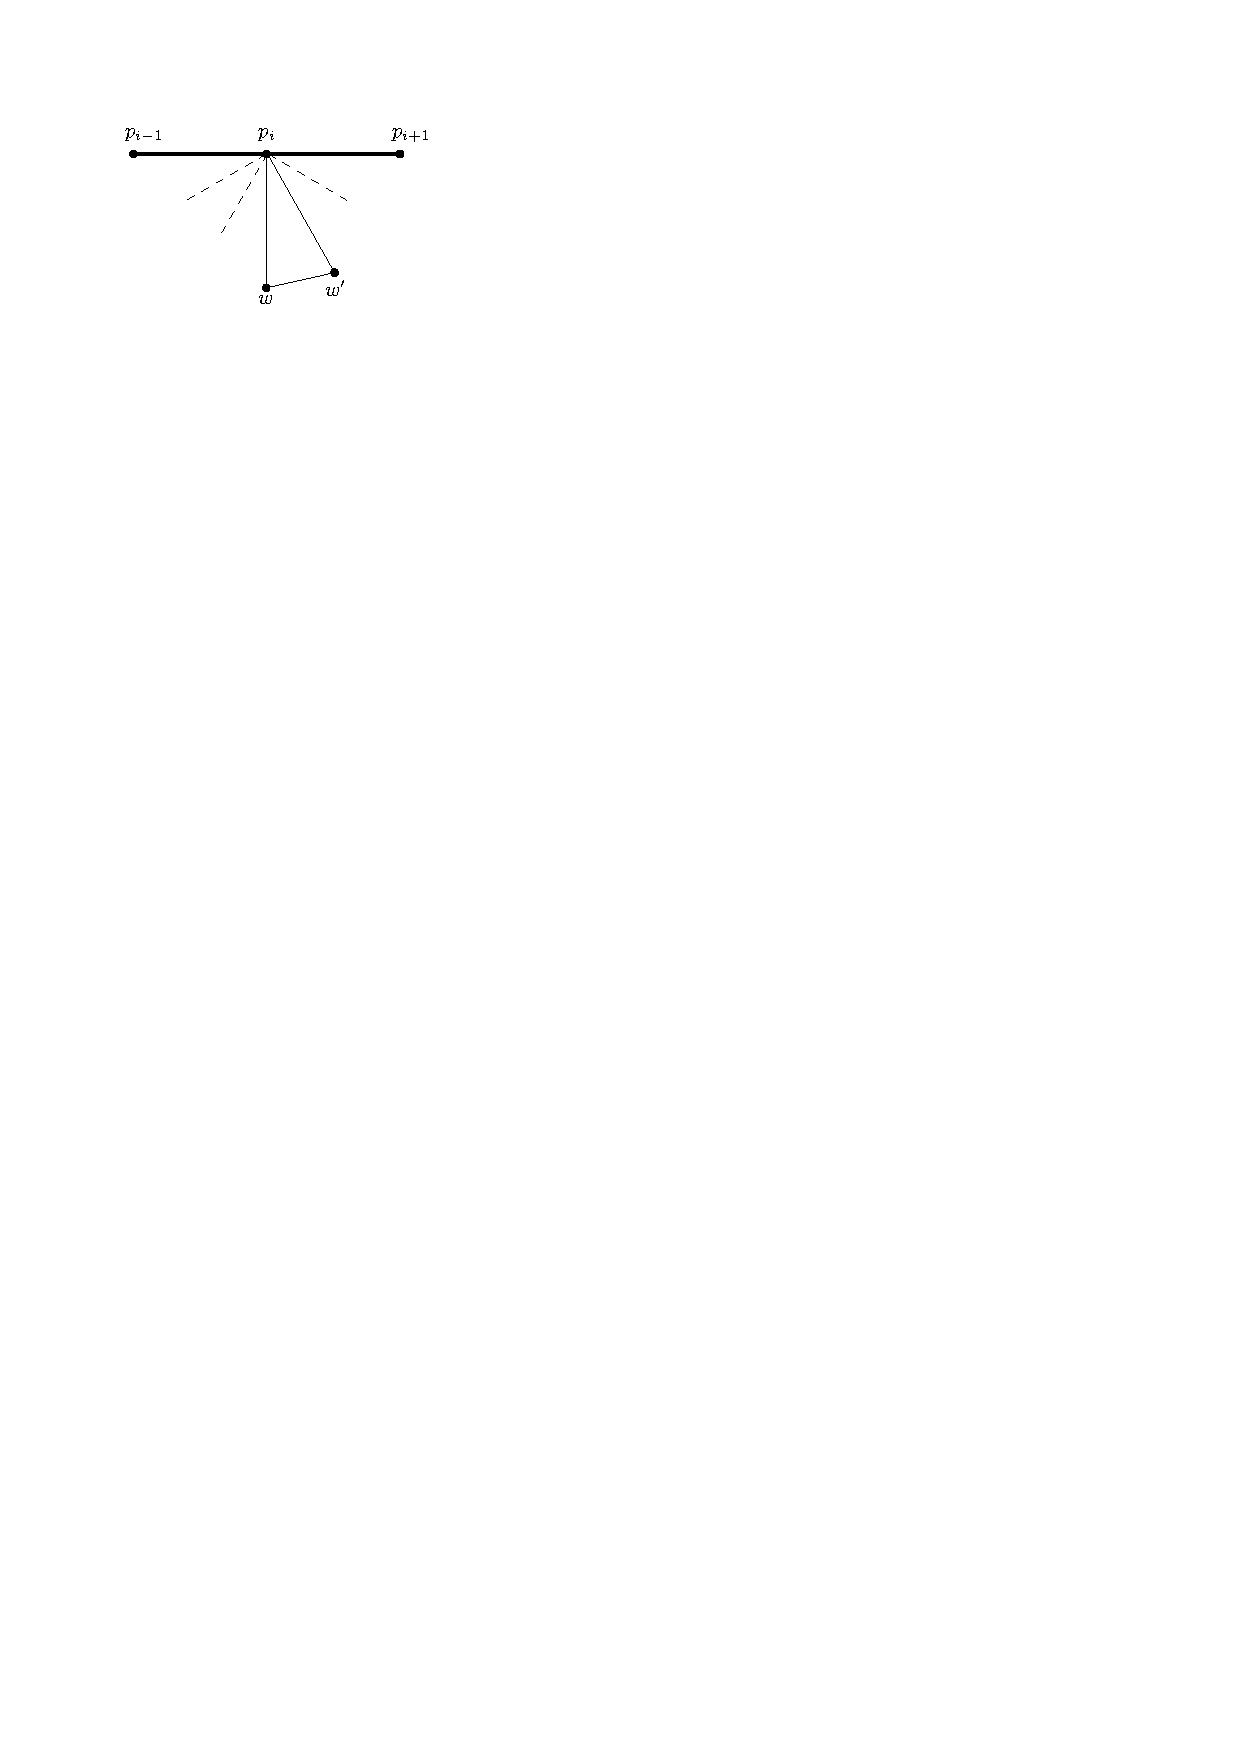
\includegraphics[width=\linewidth]{redAlgo/img/walkProofA}
            \caption{}
        \end{subfigure}%
        \begin{subfigure}[b]{0.5\linewidth}
            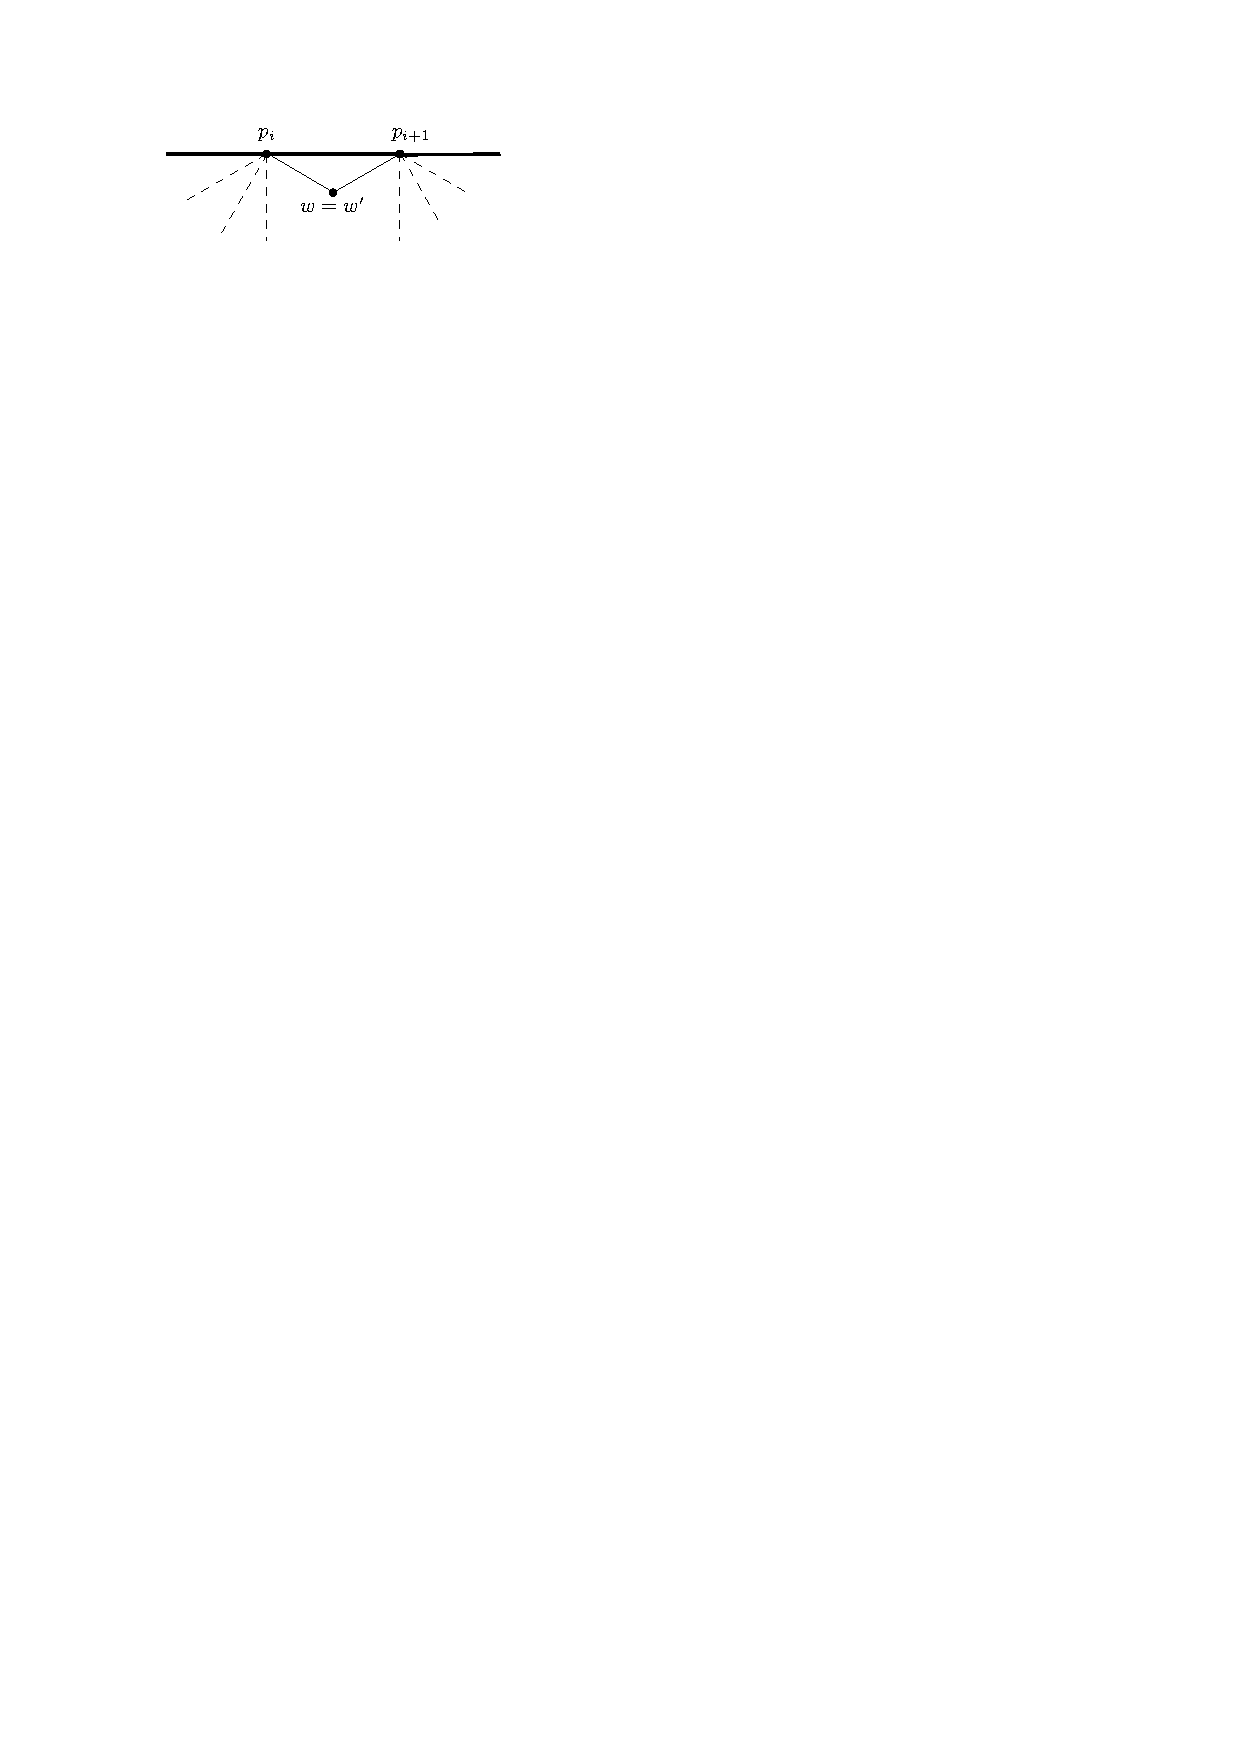
\includegraphics[width=\linewidth]{redAlgo/img/walkProofB}
            \vspace{1cm}

            \caption{}
        \end{subfigure}

          \caption{The two main cases of the proof showing that $W$ is a walk}
      \label{fig:red:walkproof}
    \end{figure}

    In case $(a)$ we note that since $w$ and $w'$ are subsequent in the rotation at $p_i$ $ww'$ is an edge by Lemma \ref{lm:prelim:rotationEdge}.

    In case $(b)$ we note that $p_i w$ and $p_i p_{i+1}$ are edges subsequent in clockwise order, hence $wp_{i+1}$ is also an edge. Hence $w$ is the first vertex adjacent to $p_{i+1}$ subsequent to $v_i$ in the clockwise rotation. Thus $w= w'$. They are duplicates and one of them must have been removed.

    Now for the edge cases: Let $x$ be the first vertex adjacent to $p_{i+1}$ and let $y$ be the last vertex adjacent to $p_{j-1}$. $p_i$ and $x$ are vertices adjacent to $p_{i+1}$ subsequent in the clockwise rotation, and hence connected by Lemma \ref{lm:prelim:rotationEdge}. In the same way $y$ and $v_j$ are subsequent vertices in the rotation at $v_n$ and hence connected.

    Hence $\W$ is a walk.
  \end{proof}


  \begin{lemma}
    \label{lm:red:neighborWalkNoncrossing}
    The right neighbor walk $W$ is a non-crosssing walk.
  \end{lemma}
  \begin{proof}
    Suppose that the right neighbor walk is crossing at a vertex $w= w_i =w_j$. Then one of $w_{j-1}$ and $w_{j+1}$ is in the clockwise interval $[w_{i-1}, w_{i+1} ]$ at the rotation at $w$. We will denote this vertex by $w'$. It is clear that $w'$ cannot be on the path unless $w'$ is $p_1$ or $p_k$. In this case however we see that $w_{i-1}$ or $w_{i+1}$ respectively couldn't have been part of the path.

    So we continue with $w'$ not on the path. All neighbors of $w$ between $w_{i-1}$ and $w_{i+1}$ in the clockwise rotation are on the path. \fxwarning{TODO make this a lemma}. So we have a series of triangles by Lemma \ref{lm:prelim:rotationEdge}. Now $w'$ must be inside one of these triangles, otherwise we would have a crossing edge (and thus a non-planar graph.) Now the triangle containing $w$ is a separating triangle.

    We conclude that $W$ must be a non-crossing walk.
  \end{proof}


  \fxnote{Actullly W rev(P)}
  \begin{lemma}
    \label{lm:red:neighbourwalkNoInteriorVertex}
    The closed non-crosing walk $WP$ has no interior vertex.
  \end{lemma}
  \begin{proof}subsequent
    The interior of $WP$ consists of only triangles with all vertices in $WP$. We can see this from the construction of the neighbor walk. Both cases in Figure \ref{fig:red:walkproof} add a triangle to the interior with all vertices in $WP$.

    Suppose there is a interior vertex. Then the triangle containing this vertex is a separating triangle.
  \end{proof}


  \begin{lemma}
    \label{lm:red:neighbourwalkChordFree}
    The left of the of a right neighbor walk and the right of the left neighbor walk are chordfree.
  \end{lemma}
  \begin{proof}
    Suppose that the right neighbor walk $W = w_1 \ldots w_k$  has a chord on the left, say between $w_i$ and $w_j$ with $i< j -1 $. There is a vertex $p_\ell \in P$ on the path such that $w_{i+1}$ is a neighbor of $p_\ell$ to the left of $p_\ell$ Consider now the following non-crossing closed walk $P w_k \ldots w_{j+1} w_j w_i w_{i-1} \ldots w_1$
    (Thick in Figure \ref{fig:red:neihbourwalkChordFree})this walk has $w_{i+1}$ in its exterior. But then $p_\ell w_{i+1}$ is a crossing edge. Which is forbidden.

    \begin{figure}[h]
      \centering
      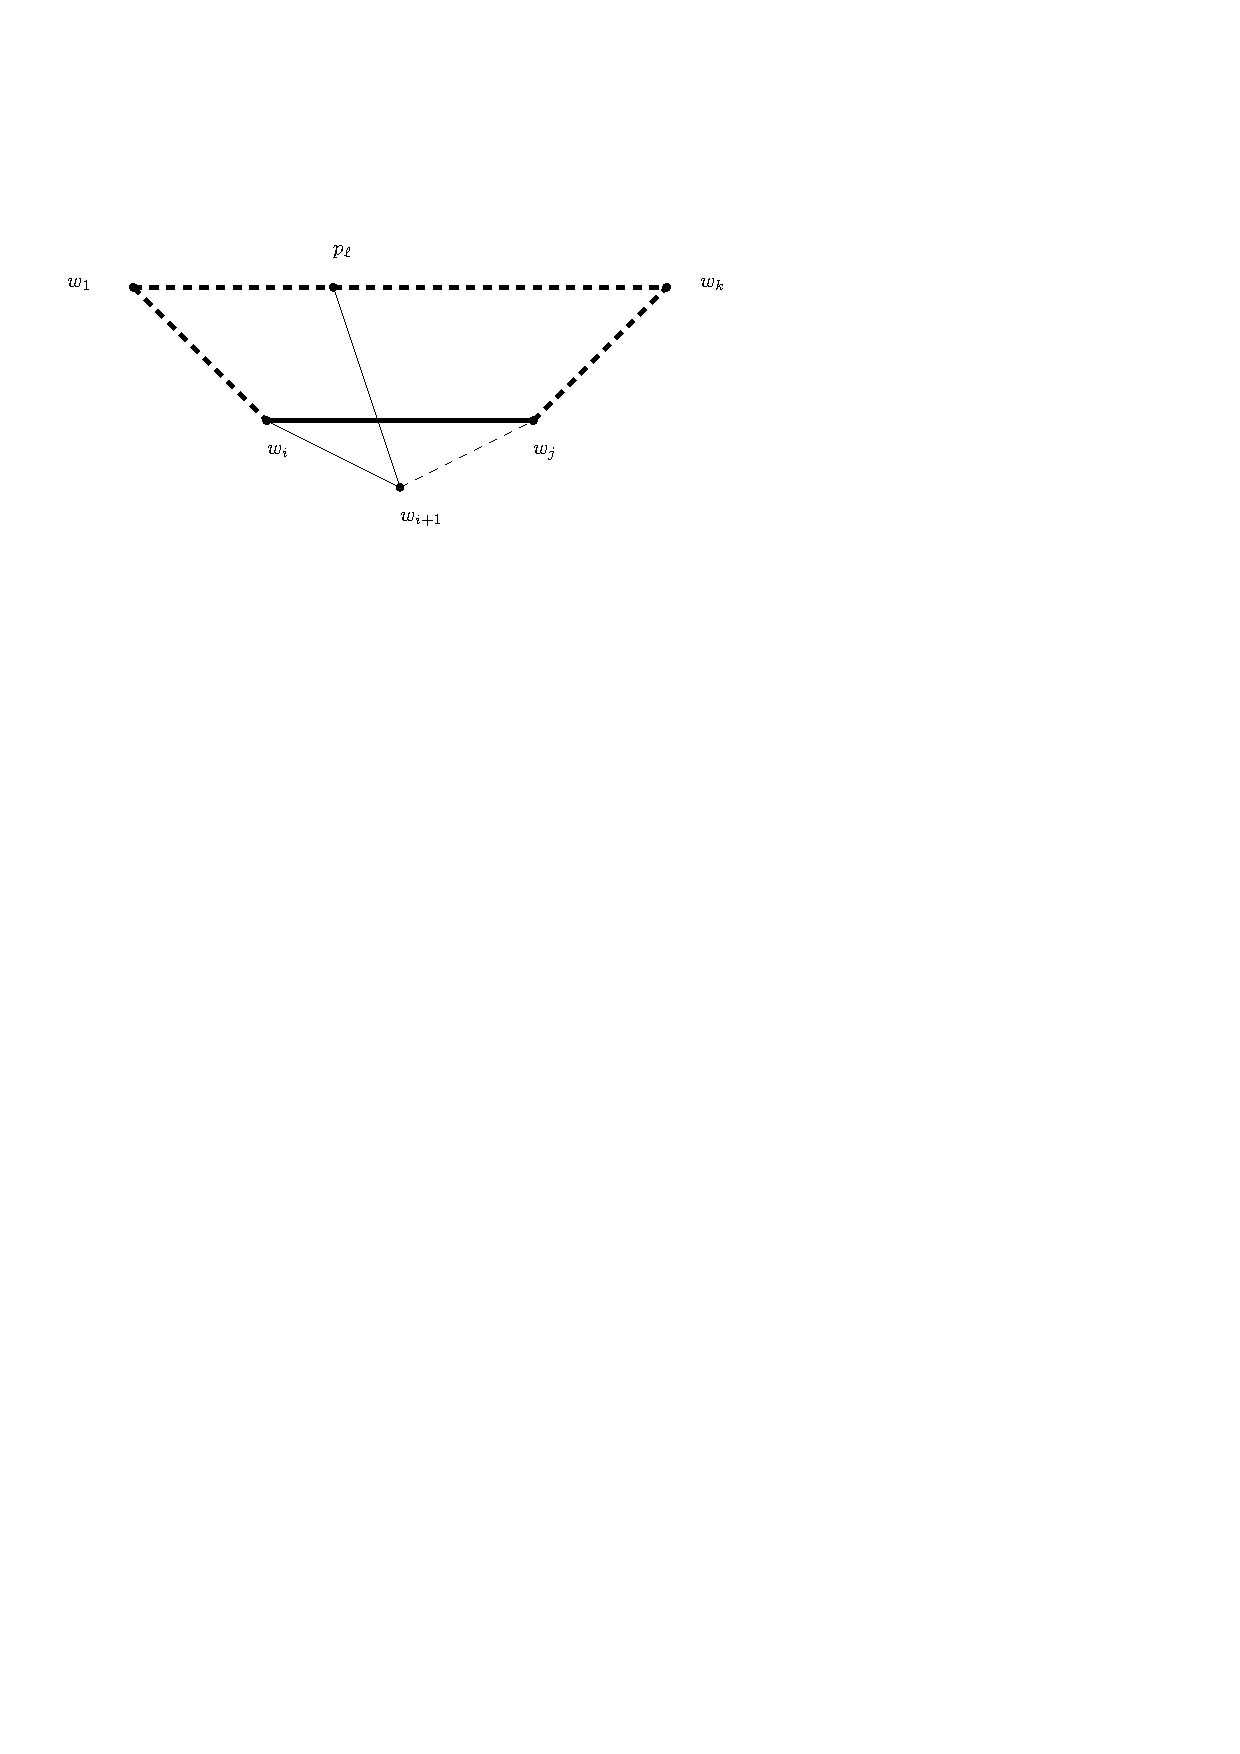
\includegraphics[scale=1]{redAlgo/img/neighbourWalkChords}
      \caption{The construction in the proof of Lemma \ref{lm:red:neighbourwalkChordFree}}
      \label{fig:red:neihbourwalkChordFree}
    \end{figure}
  \end{proof}

  \fxnote{Alternate proof based on   ($\W$ being oriented from $\pW$ to $\pE$), since if it would lie on the left of $\W$ the vertices $w_{i+1},\ldots, w_{j-1}$ would not have been chosen in the construction of the prefence.}

\subsection{Outline}
  We will assume we have no separating $3$ or $4$ cycles.

  To describe the algorithm two more definitions are necessary

  \begin{defi}[Prefence]
  A prefence $\W$ is a interior walk of $\C$ starting at $v_i \in \C$ and ending at $v_j \in \C$ a both adjacent to $\pS$
  \begin{enumerate}
   \renewcommand*{\labelenumi}{(P\arabic{enumi})}%
   \renewcommand*{\theenumi}{(P\arabic{enumi})}%
    \item  $\C_\W$ Has no interior vertex
    \label{p:noInteriorVertex}
    \item  $\W$ has no chords on the left
    \label{p:Cchordfree}
    \item  $\restC{\W}$ has no chords on the right
    \label{p:Wchordfree}

  \end{enumerate}
  \end{defi}


  We enforce these conditions because they imply \ref{e:crossingEdges} as we will show in Lemma \ref{lm:red:regularPrefenceIsFence}.

  For a walk however the interior is not clearly defined. \fxnote{Use a non-crossing walk}

  \begin{defi}[Fence]
    A fence is a valid path starting and ending at a vertex adjacent to $S$
  \end{defi}

  \fxnote{ expand on naming/reasons of fence}



  The algorithm will receive as input a extended graph $\ext G$ and will return a regular edge labeling such that all red faces are $(1-\infty)$ using a sweep-cycle approach inspired by Fusy \cite{Fusy2006}.

  We will start by creating a prefence $W$. This may not be a valid path, it does not even have to be a path. During the algorithm we will make a number of moves that will turn this prefence into a fence. In each move we shrink $C$ by employing a valid paths and change the prefence.

\subsection{Finding a initial prefence}
  Let $v_i$ denote all the vertices of $\cpath$ in the following order $\pW =  v_1 \  v_2 \  \ldots v_{n-1} \  v_n = \pE$.
  Some intervals of these vertices will be adjacent to $\pS$. However, they can not be all adjacent to $S$ since then the sweepcycle would be non-separating since we can not have separating triangles. We denote by $v_i$ the last vertex of fist interval of vertices adjacent to $S$ and by $v_j$ the first vertex of the second interval.
  As candidate walk we will take the right neighbor path of $C\sm{S, v_1, \ldots v_{i-1}, v_{j+1}, \dots v_n}$.
  \fxnote{beter notation}

  \begin{lemma}
    \label{lm:red:isPrefence}
  The collection $W$ described above is a prefence.
  \end{lemma}
  \begin{proof}
  $W$ is a walk by lemma \ref{lm:red:neighborWalk}.

  We note \ref{p:noInteriorVertex} holds due to Lemma \ref{lm:red:neighbourwalkNoInteriorVertex}

  We note \ref{p:Cchordfree} holds due to invariant \ref{i:noChords}.

  We note \ref{p:Wchordfree} holds due to Lemma \ref{lm:red:neighbourwalkChordFree}

  \end{proof}

  We then orient $\W$ from $v_i$ (the vertex closest to $\pW$)to $v_j$ (the vertex closest to $\pE$) and denote it's vertices by $w_1 \ldots w_k$.

\subsection{Irregularities}
  We will distinguish two kinds of \emph{irregularities} in a prefence.
  \begin{enumerate}
    \item The candidate walk is non-simple in a certain vertex. That is, if we traverse the sequence of vertices in $\W$ we see that $w_i = w_j$ for some $i<j$.
    \item The candidate walk has a chord on the right. That is, there is an edge $w_i w_j$ on the right of $\W$ with $i<j$ and $i$ and $j$ not subsequent (i.e. $i < j-1$).
  \end{enumerate}

  Note that we can not have a chord can on the left of $\W$ by Lemma \ref{lm:red:neighbourwalkChordFree}.


  \begin{lemma}
    \label{lm:red:regularPrefenceIsFence}
    If a prefence has no irregularities it is a fence.
  \end{lemma}
  \begin{proof}
    We will show that all the requirements of being a valid path are met.
   \begin{itemize}
     \item [Path] Let us begin by noting that since there are no non-simple points we have a path and not just a walk.

     \item[\ref{e:noS}] It is clear that both $w_1$ and $w_k$ are not $\pS$ by the construction of the candidate walk.

     \item[\ref{e:longBorders}] For $\W$ or $\restC \W$ to have only one edge we need to have that $v_i v_j$ is an edge. However, $v_i v_j$ can not be an edge in $\C$ since $v_i$ and $v_j$ are from different intervals of vertices adjacent to $\pS$. It can also not be an edge in $\ext G \setminus \C$ since that would be a chord of the cycle and these do not exist by Invariant \ref{i:noChords}

     \item[\ref{e:crossingEdges}]
     This holds because every interior edge that does not lead to an interior vertex, nor is a chord of $\W$ or $\restC{\W}$ is of the required type. These three requirements are forces by \ref{p:noInteriorVertex}, \ref{p:Wchordfree} and \ref{p:Cchordfree} respectively.

     \item[\ref{e:noNewChord}] The cycle $\C'$ only changes between $v_i$ and $v_j$. There can be no chord with one vertex from cycle $\C \setminus \restC{\W}$ and one from $\W$ since such a chord would cross $\pS v_i$ or $\pS v_j$. There is no chord with two vertices in $\W$ since that would be a irregularity and there is no chord with two vertices from $\C \setminus \restC{\W}$ by Invariant \ref{i:noChords}.
   \end{itemize}
   Hence, if $\W$ has no irregularities it is a valid path.

   Furthermore, $\W$ is a path starting and ending at a vertex adjacent to $\pS$ because it is prefence. And thus it is a fence.
  \end{proof}


  \begin{defi}[Range of a irregularity]
  For a non-simple point \fxnote{Is it better to call this a non-simple point or a non-simple vertex?} $w_i = w_j$ with $i<j$ has \emph{range} $\braces{i, \ldots, j} \subset \N$.
  A chord $w_i w_j$ with $i< j-1$ has \emph{range} $\braces{i, \ldots, j} \subset \N$.
  \end{defi}

  Note that a chord can not have the same range as a non-simple point since then $w_i w_j$ will be a loop and we are considering simple graphs. Furthermore two chords have different ranges because we otherwise have a multiedge. Two nonsimple points with the same range are, in fact, the same. This leads us to the following remark.
  \begin{remark}
  \label{rk:diffIregDiffRange}
  Distinct irregularities have distinct ranges.
  \end{remark}

  \begin{defi}[Maximal irregularity]
  A irregularity is maximal if it's range is not contained\footnote{Because of Remark \ref{rk:diffIregDiffRange} being contained is the same as being strictly contained} in the range of any other irregularity.
  \end{defi}

  \begin{lemma}
  \label{lm:rangeOverlap}
  Maximal irregularities have ranges whose overlap is at most one integer.
  \end{lemma}
  \begin{proof}
  We let $I$ and $J$ denote two distinct maximal irregularities with ranges $\braces{i_1, \ldots i_2}$ and $\braces{j_1, \ldots, j2}$. Let us for the moment suppose that $I$ and $J$ have ranges that overlap more then one integer. Since $I$ and $J$ are both maximal their ranges can not be contained in each other.

  Without loss of generality we thus have $i_1 < j_1 < i_2 < j_2$.

  Now two chords to the right of $\W$ would cross each other but we have a planar graph so this can not be the case.

  Now let us without loss of generality suppose that $I$ is a non-simple point. A non-simple point $w_{i_1} = w_{i_2}$ is adjacent to two ranges of vertices in $\cpath$. $v_a \ldots v_b$ and $v_c \ldots v_d$
  then $\tilde{C} = w_{i_1} v_b \ldots v_c$ is a cycle. And because of the rotation at $w_{i_1} = w_{i_2}$ we have that $w_{i_{1 +1}}, \ldots, w_{i_{2 -1}}$ are inside this cycle while $w_1 \ldots w_{i_1 -1}$ and $ w_{i_2 +1} \ldots w_k$ are outside the cycle. See Figure.
    \fxnote{We could add figure to clarify.}

  Now if $J$ is a chord we have $\tilde{C}$, which can not be. If $J$ is also a nonsimple point this would imply that the vertex $w_{j_i} = w_{j_2}$ is at the same time inside and outside $\tilde{C}$ which is clearly impossible.
  \end{proof}

\subsection{Moves}
  \newcommand{\U}{\scr U}
  The algorithm will remove these irregularities by recursing on a subgraph for each maximal irregularity. We shrink the cycle $\C$ with every valid path that is found in the recurrence, in the order they are found. Afterwards we update the prefence by removing $w_{i+1}, \ldots, w_{j-1}$. In subsection \ref{ss:validity} we will show that the updated prefence is a prefence for the updated cycle $\C$.


  We will first show how to remove these maximal irregularities in Subsections \ref{ss:chords} and \ref{ss:nonsimplePoints}. That is, we show which \emph{recursion subgraph} $H$ we recurse upon for both kinds of irregularity. Furthermore we show that these subgraphs suffice the requirements of the algorithm.

  Afterwards, in subsection \ref{ss:validity} we will make sure that the subgraphs we recurse upon are edge-disjoint. That is, they only overlap in border vertices.

  It is worth noting that other irregularities contained in such a maximal irregularity are solved in the recurrence.

  \subsubsection{Chords}
    \label{ss:chords}
    If we encounter a chord we will extract a subgraph and recurse on this subgraph. A chord $w_iw_j$ has a triangular face on the left and on the right (like every edge). The third vertex in the face to the left will be called $x$. $x$ is not necessarily distinct from $w_{i+1}$ and/or $w_{j-1}$ but this is also not necessary for the rest of the argument. \fxnote{We might also work these out in a Figure.}

    The vertex $v_a$ on the cycle is uniquely determined as the vertices adjacent to both $w_i$ and $w{i+1}$. In the same way $v_b$ is the unique neighbor of $w_{j-1}$ and $w_j$.

    We will describe a walk $\U$ running from $v_a$ to $v_b$. This path consists of all vertices adjacent to $w_i$ in clockwise order from $v_a$ (inclusive) to $x$(inclusive) and subsequently all vertices adjacent to $w_j$ in clockwise order from $x$ (exclusive) to $v_b$ (inclusive). This path is given in bold in Figure \ref{fig:removeChord}.

    Note that $\U$ is the left neighbor walk of $v_a w_i w_j v_b$.

    \begin{lemma}
    $\U$ is a chordfree path
    \end{lemma}
    \begin{proof}
    We note that $\U$ is a walk due to Lemma \ref{lm:red:neighborWalk}.

    $\U$ cant have a non-simple point $x'$ since it would have to be connected to at least two vertices. However a vertex $x'$ that is distinct from $x$ and is connected to both $w_i$ and $w_j$ will induce a separating triangle $w_i x' w_j$. $\U$ also can not be nonsimple at $x$ since $x$ is the the third vertex of the triangular face $w_i w_j x$. Hence $\U$ is a path.

    $\scr U$ can not have chords $u_i u_j$ since they would either induce a separating $3$- or $4$-cycle either $w_i u_i u_j$ or $w_j u_i u_j$ or $w_i u_i u_j w_j$ depending on the vertex adjacent to $u_i$ and $u_j$.
    \fxnote{We use that we have no 4-cycles here}
    \end{proof}


    We take $\intplus(\C_\U)$ as the subgraph $H$. We then take the tight extension at $v_a$ and $v_b$. We will then recurse on this graph $\tightext H$. See also Figure \ref{fig:removeChord}. Since $\C$ is chordfree by invariant \ref{i:noChords} so is $\restC{\U}$. We have also just shown that $\U$ is chordfree. So $\tightext H$ is indeed defined.
    Furthermore, since $H$ is a induced subgraph of $G$, $\tightext H$ contains no separating $4$-cycles not involving the poles.
    \fxfatal{ALSO WITH POLES IS STILL BAD}

    We update the prefence by removing $w_{i+1}, \ldots, w_{j-1}$.

    \begin{figure}[h!]
    \centering
    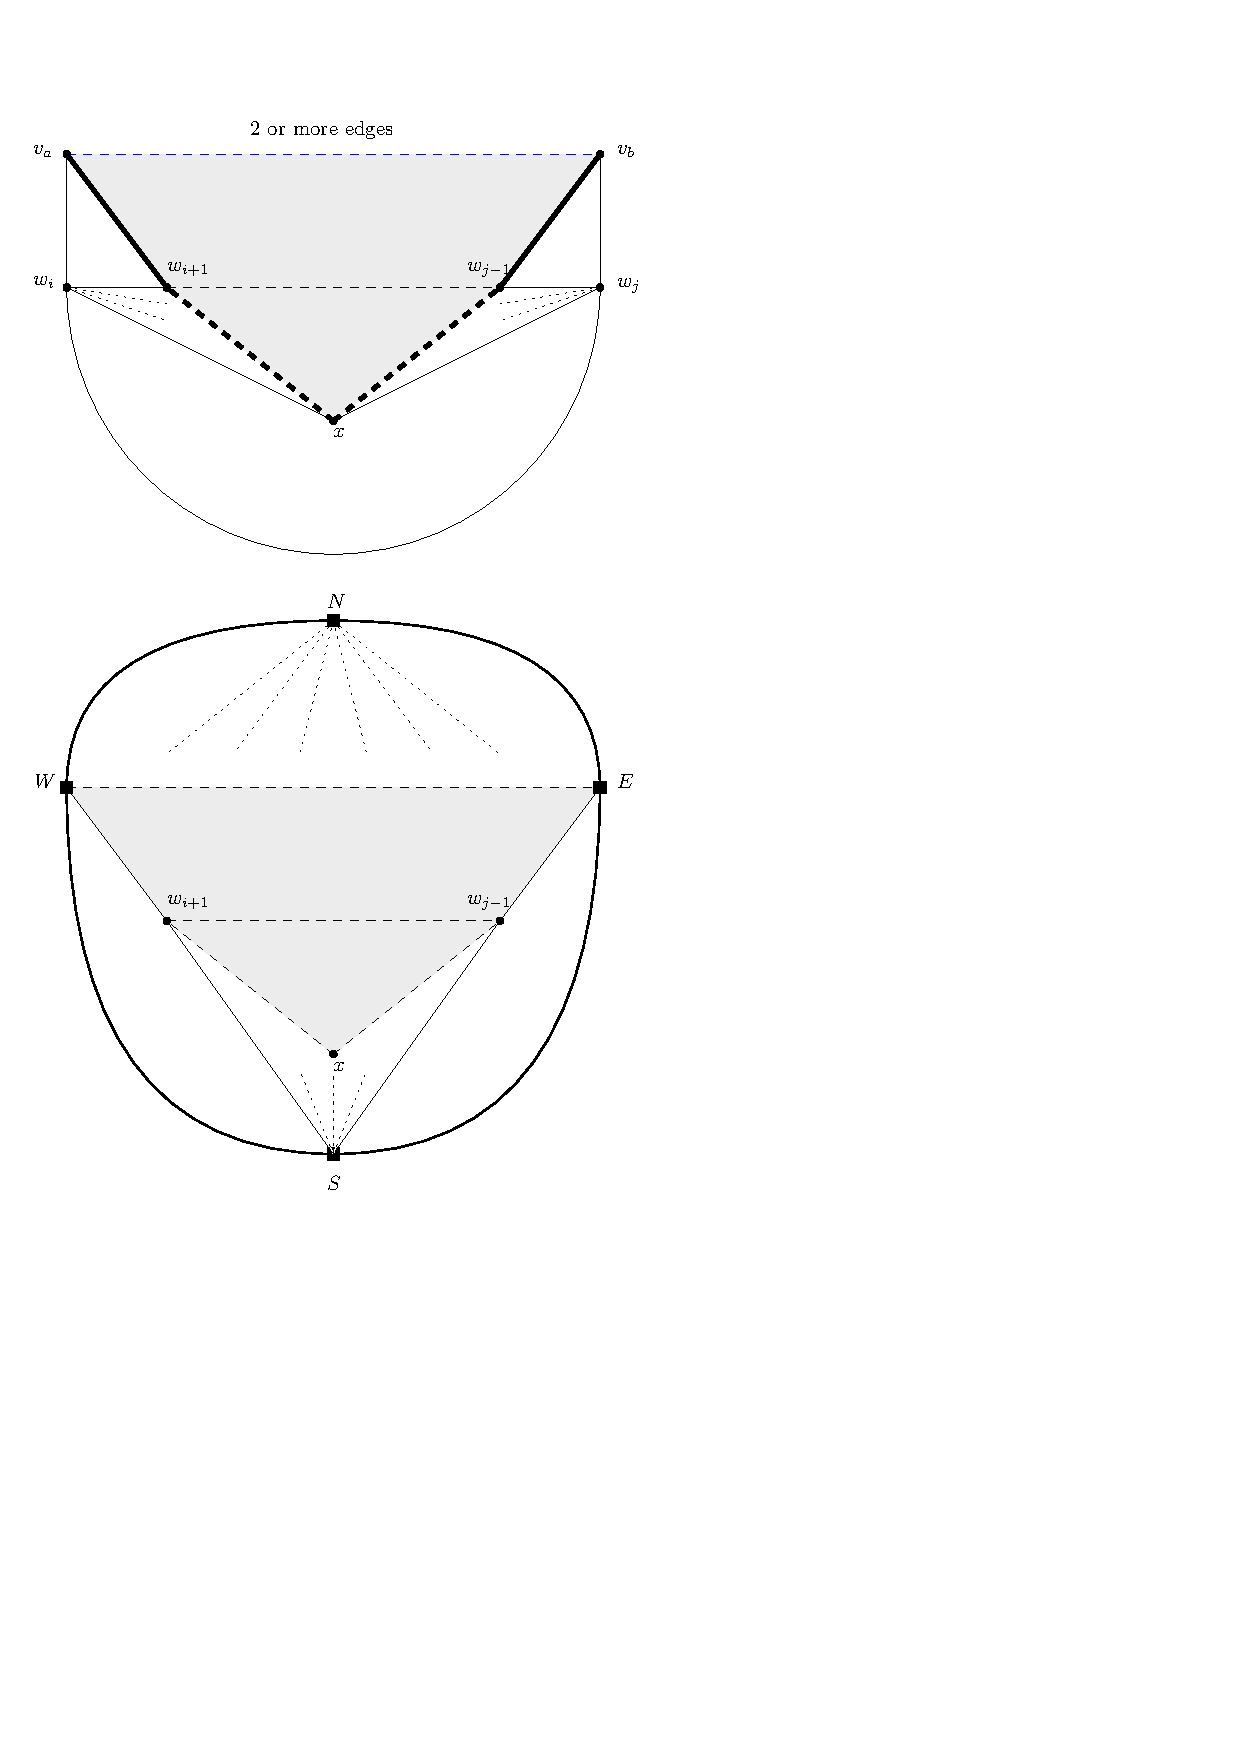
\includegraphics[scale=1]{redAlgo/img/removeChord}

    \caption{Removing a chord
        \label{fig:removeChord}}
    \end{figure}

  \subsubsection{Nonsimple points}
    \label{ss:nonsimplePoints}
    Removing a non-simple point is done is a similar manner.

    The vertex $v_a$ on $\C$ is uniquely determined as the vertices adjacent to both $w_i=w_j$ and $w{i+1}$. In the same way $v_b$ is the unique neighbor of $w_{j-1}$ and $w_j=w_i$. Note that it may be that $w_{i+1} = w{j-1}$ this does not matter for the rest of the argument. \fxnote{We may show this in a figure.}

    We will describe a walk $\scr U$ running from $v_a$ to $v_b$. This path consists of all vertices in the rotation at $w_i=w_j$ from $v_b$ (inclusive) to $v_a$(inclusive). This path is given in bold in Figure \ref{fig:removeNonSimplePoint}.

    Note that $\U$ is the left neighbor walk of $v_a w_i v_b$.


    \begin{lemma}
    $\U$ is a chordfree path.
    \end{lemma}
    \begin{proof}
      We note that $\U$ is a walk due to Lemma \ref{lm:red:neighborWalk}.

      If we orient $\U$ from $v_a$ to $v_b$  we see that $\U$ can not have a non-simple point on the left by construction and by the right since such a point would have edges to at least two vertices on the right. However every vertex can only be connected to $w_i=w_j$. Hence $\U$ is a path.

      $\U$ can not have chords on the right of the path by the way we construct $\U$. Furthermore $\scr U$ can not have chords $u_i u_j$ on the left since they would either induce a separating $3$-cycle $w_i u_i u_j$.
    \end{proof}


    We then take $\intplus(\C_\U)$ as the subgraph $H$.

    We then take the tight extension of $H$ at $v_a$ and $v_b$ to recurse on. See also Figure \ref{fig:removeNonSimplePoint}. Since $\C$ is chordfree by Invariant \ref{i:noChords} so is $\restC{\U}$. We have also just shown that $\U$ is chordfree. So $\tightext H$ is indeed defined. Furthermore, since $H$ is a induced subgraph of $G$, $\tightext H$ contains no separating $4$-cycles not involving the poles.

    \fxfatal{ARRARGH also poles are not allowed}

     We update the prefence by removing $w_{i+1}, \ldots, w_{j-1}$ and we also recognize that $w_i = w_j$ is now a duplicate subsequent occurrence of the same vertex. So we also remove $w_j$.

    \begin{figure}[h!]
    \centering
    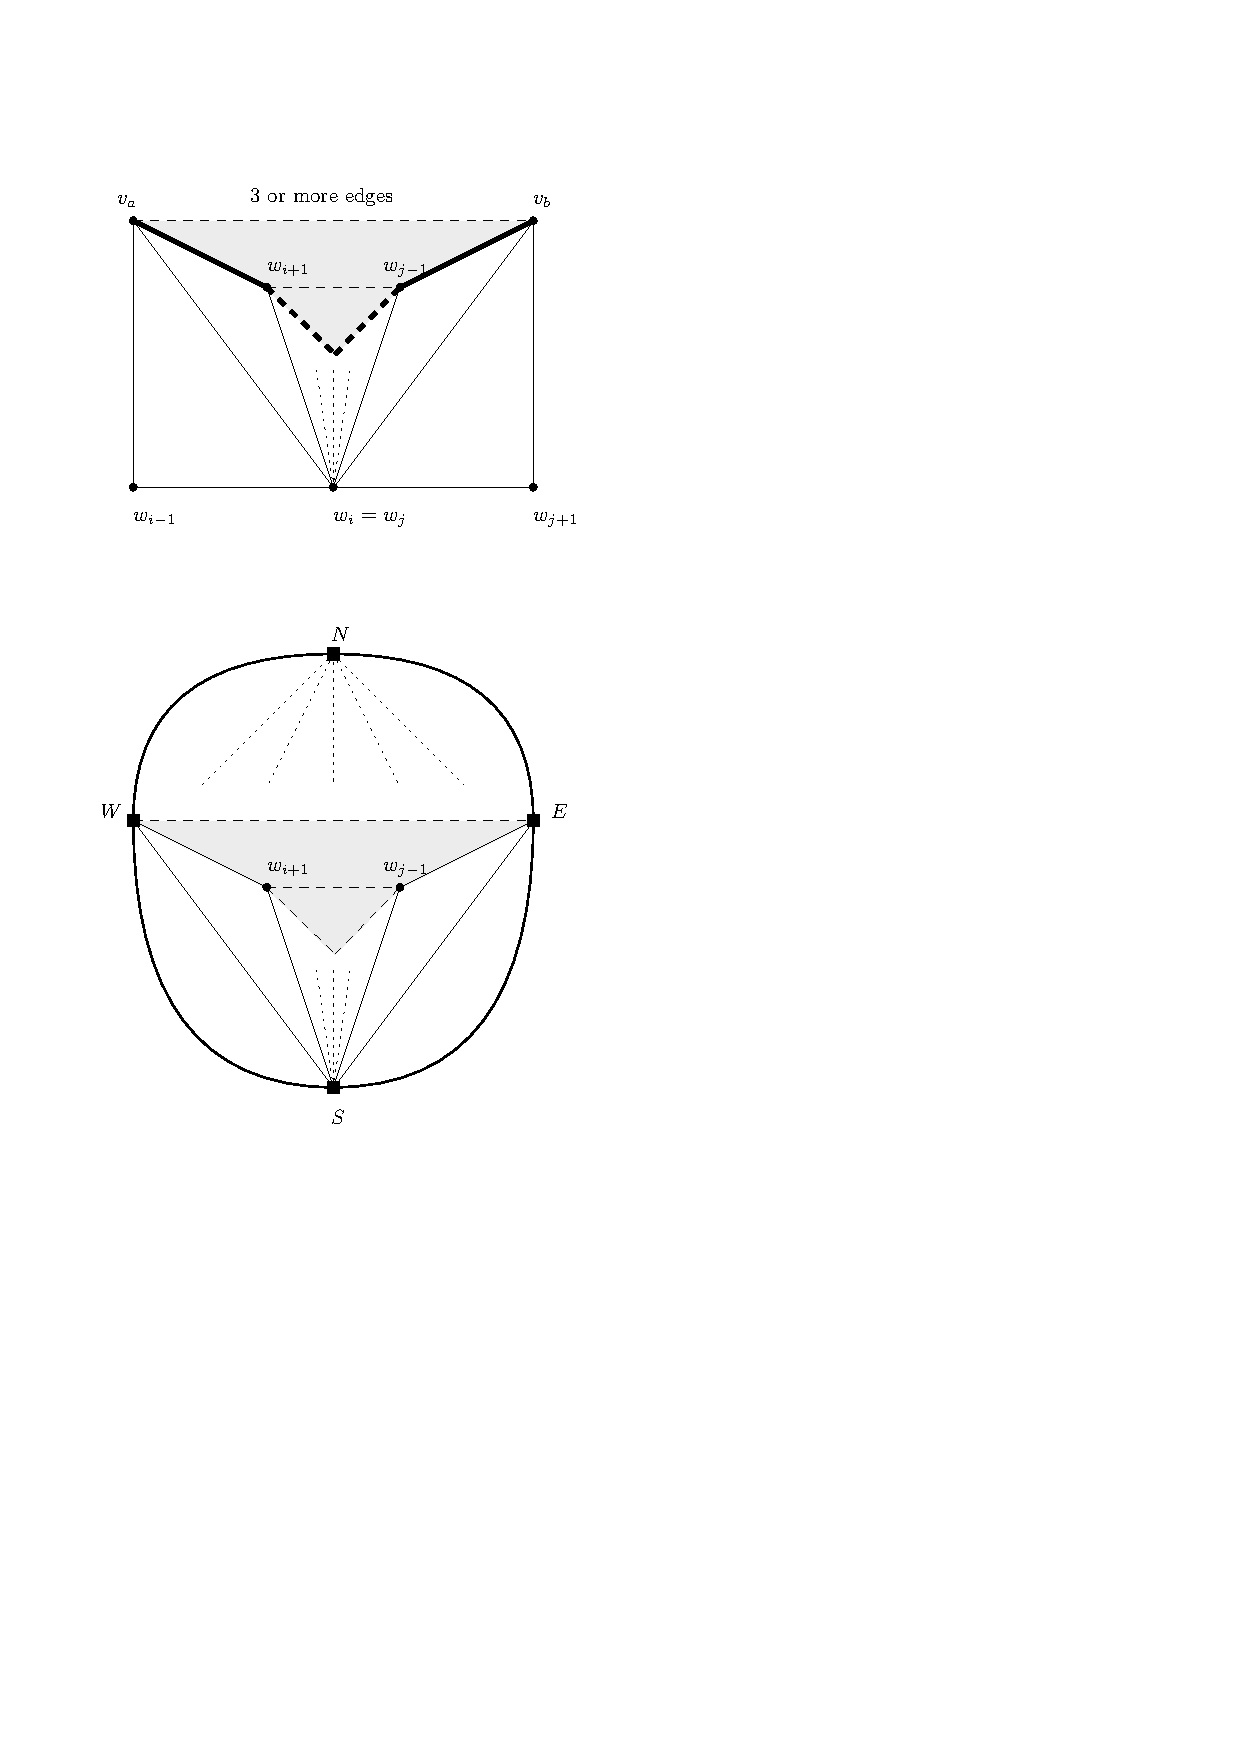
\includegraphics[scale=1]{redAlgo/img/removeNonSimplePoint}

    \caption{Removing a non-simple point
        \label{fig:removeNonSimplePoint}}
    \end{figure}

\subsubsection{Validity}
  \label{ss:validity}

  \begin{lemma}
  After doing a move the updated prefence $\W'$ is a prefence for the updated cycle $\C'$
  \end{lemma}
  \begin{proof}
    We want to show that the three properties of a prefence again hold for $\W'$.

    We will first show \ref{p:noInteriorVertex} still holds.
    We note we can cut the interior of $\C'_{\W'}$ into
    three parts: $w_1 \ldots w_i v_a v_{a-1} \ldots v_{i+1} w_1$, $\U w_j w_i$ (or $\U w_i$) and $w_j \ldots v_j \ldots v_{b+1} v_b w_j$.
    Note that the first and last part are free from interior vertices because they already were before the move by \ref{p:noInteriorVertex}.
    As for the middle part since $\U$ is the left neighbor path of $v_a w_i w_j v_b$ (or $v_a w_i v_b$) this is also without interior vertices by Lemma \ref{lm:red:neighbourwalkNoInteriorVertex}.

    Since in the recursion the cycle $\C$ is only updated with valid paths it remains a valid cycle. Thus Invariant \ref{i:noChords} still holds for $\C'$ and thus implies \ref{p:Cchordfree}.

    Furthermore we can easily see \ref{p:Wchordfree} holds. Suppose we have a chord on the left of $\W'$ then this would already have been a chord of $\W$ however $\W$ has no chords due to \ref{p:Wchordfree}.
  \end{proof}

  \begin{lemma}
  Let $H_I$ and $H_J$ be two recursion subgraphs for different maximal irregularities $I$ and $J$. Then $H_I$ and $H_J$ are edge disjoint.
  \end{lemma}
  \begin{proof}
    Maybe the best proof is that since maximal ranges of irregularities overlap at most $1$ then the cycles $v_{a_I} \ldots v_{b_I} w_{j_I} w_{i_I}$  and  $v_{a_J} \ldots v_{b_J} w_{j_J} w_{i_J}$
    with $v_{a_I}$ being the unique neighbor on the cycle of $w_{i_I}$ and $w_{i_I+1}$ and ....
    do not cross

    Then the left neighbor paths $U_I$ and $U_J$ are edge disjoint

     \fxwarning{TODO fix this lemma}

  \end{proof}

\subsection{Correctness}
  As long as the interior of $\C$ is nonempty we can find a prefence. And thus we find valid paths. Since we continuously shrink the cycle with valid paths we end up with a regular edge labeling.
  See core algorithm

  The algorithm finishes because it keeps on recursing and shrinking until no graph is left.

  \subsubsection{The red faces}
  Let us then argue that the red faces are all $(1-\infty)$ faces, corresponding to one-sided vertical segments. As is shown in Lemma \ref{lm:zInRedFace} it is sufficient to show no two vertices subsequent on a blue path are first a merge and then a split or vice versa.

  We will show the following
  \begin{lemma}
    A split or merge always happens on a vertex that is adjacent to $S$ for some recursion.
  \end{lemma}

  \begin{proof}
    Every valid path we shrink the cycle by is found as a fence on some recursion level. In this recursion level both $w_1$ and $w_k$ are adjacent to $S$.
  \end{proof}

  \begin{lemma}
    \label{lm:pathsStayOnRecursionLevel}
    A path starting at a certain recursion level will stay at that recursion level. It may share vertices with the north boundary of a lower recursion level but never with the south boundary.
  \end{lemma}
  \begin{proof}
    A valid path can never leave the subgraph $H$ in which its start- and end-vertex are located. Because it is found as a fence in this subgraph. It can also never run trough a graph $H'$ on a lower recursion level (except for the north boundary path)  because in every move the vertices of the prefence in $H'$ are deleted.
  \end{proof}

  Recall that all our valid paths are oriented from a start vertex to end vertex.

  \begin{lemma}
    A split can not directly be followed by a merge along any valid path during the algorithm.
  \end{lemma}
  \begin{proof}
    One of paths after the split is no longer on the south boundary of this subgraph $H$, nor on the south boundary of any other subgraph by Lemma \ref{lm:pathsStayOnRecursionLevel}. This path hence can not contain a merge.

    The other path still potentially follow the south boundary. However merging from the southward side of the path is impossible by Lemma \ref{lm:pathsStayOnRecursionLevel} from the northward side is equally impossible since the split and merge have to be neighboring vertices in the rotations of these vertices and thus the path $\P$ that merged must also join again.

    But then it is not a valid path.
  \end{proof}

  However for a blue $Z$ to occur there has to be a valid path that first has a split and then has a merge. Since this can not be all red faces must have only $2$ edges on at least one side. Hence the regular edge labeling this algorithm produces corresponds to a vertically one-sided rectangular dual.


  \fxnote[inline, nomargin]{Show how the algorithm works with some cool examples: For example:    The multiple non-simple point $v_i = v_j =v_k$;   Example of page $F1$;  Example with lots of layered chords  }
